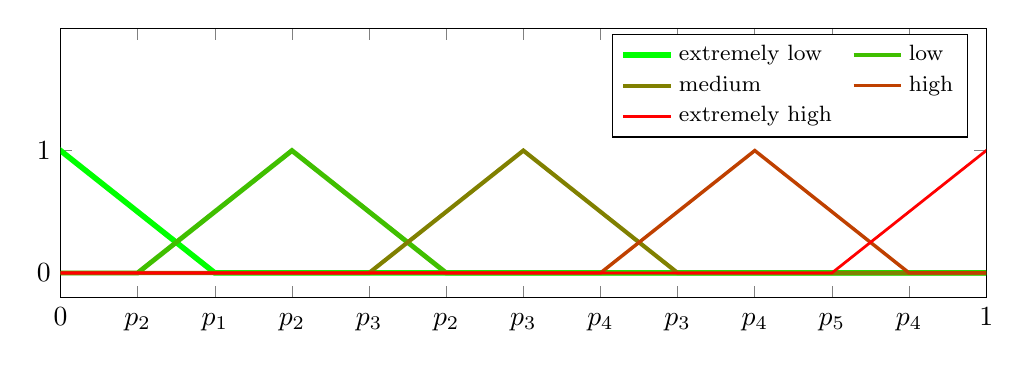
\begin{tikzpicture}
    \linespread{1}

    \pgfmathsetmacro\fuzzywidth{1.3333}

    \begin{axis}[
        width            = 1.1\textwidth,
        height           = 5cm,
        legend columns   = 2,
        legend style     = {legend cell align = left, font = \footnotesize, /tikz/column 2/.style={column sep=5pt}},
        xtick            = {0, 0.33333, ..., 4},
        xticklabels      = {$0$, $\pl{p}_2$, $\pu{p}_1$, $p_2$, $\pl{p}_3$, $\pu{p}_2$, $p_3$, $\pl{p}_4$, $\pu{p}_3$, $p_4$, $\pl{p}_5$, $\pu{p}_4$, 1},
        xticklabel style = {text height = 1.5ex},
        xmin             = 0,
        xmax             = 4,
        ytick            = {0, 1},
        yticklabels      = {$0$, $1$},
        ymax             = 2]

        \pgfplotsinvokeforeach{0,25,...,100}{
        \addplot[draw = red!#1!green, line width = 2pt-#1*0.01pt]
            coordinates {
                (-1, 0)
                (0.04*#1 - 0.5*\fuzzywidth, 0)
                (0.04*#1, 1)
                (0.04*#1 + 0.5*\fuzzywidth, 0)
                (6, 0)
            };
        }

        \legend{extremely low, low, medium, high, extremely high}
        \end{axis}
\end{tikzpicture} 